\documentclass{article}
\usepackage[english, russian]{babel}
\usepackage[T2A]{fontenc}
\usepackage[utf8]{inputenc}
%
\usepackage[russian]{babel}
\usepackage{graphicx}
%\graphicspath{{image constructors/}}
%\DeclareGraphicsExtensions{.png,.svg,.eps}
\usepackage[a4paper,left=2.5cm, right=1.5cm, top=2.5cm, bottom=2.5cm]{geometry}
\usepackage{amsfonts}
\usepackage{amsmath}
\usepackage{amssymb}
\usepackage{autonum}
%\usepackage{hyperref}

\newtheorem{deftext}{определение}
\newtheorem{theoremtext}{теорема}
\newtheorem{commenttext}{замечание}
\newtheorem{exampletext}{пример}

\begin{document}
	\large
	\section{модуль ontology.py}
	Здесь хранится классы для хранения и взаимодействия с онтологией
	
	\subsection{класс Ontology}
	этот класс хранит и обрабатывает онтологию.
	
	Ограничения на онтологию:
	\begin{itemize}
		\item все классы имеют различные названия
		\item все отношения исходящие из 1 класса имеют одинаковое название
		\item все сущности из одного класса имеют различные названия
		\item фиксированное отношение между фиксированными сущностями может существовать только в единственном виде(без множественности)
	\end{itemize}\ \\
	
	\begin{enumerate}
	\item def \_\_init\_\_(self, fileName=None)
		\begin{itemize}
			\item fileName - файл с сохраненной онтологией с папке ./saved/
		\end{itemize}
		конструктор, создающий пустую онтологию при fileName=None
	
	\item def addClass(self,className)
	\begin{itemize}
		\item className - название класса
	\end{itemize}
	добавление нового класса, с генерацией ошибки при существовании добавляемого класса
	
	\item def changeClass(self,oldClassName, newClassName)
	\begin{itemize}
		\item oldClassName - старое название класса
		\item newClassName - новое название класса
	\end{itemize}
	изменение названия класса, с генерацией ошибки при существовании нового класса или отсутствии старого класса
	
	\item def deleteClass(self,className,deep=False)
	\begin{itemize}
		\item className - название класса
		\item deep - метка для глубокого удаления
	\end{itemize}
	удаление класса, с генерацией ошибки при несуществовании класса, при глубоком удалении со всеми связями на него и из него и с генерацией ошибки при наличии связей
	
	\item def addRelationship(self, relationshipName, outClassName, inClassName)
	\begin{itemize}
		\item relationshipName - название отношения
		\item outClassName - название выходного класс
		\item inClassName - название входного класс
	\end{itemize}
	создание отношения, с генерацией ошибки при несуществовании одного из классов или уже существовании отношения
	
	\item def changeRelationship(self, oldRelationshipName, newRelationshipName, outClassName)
	\begin{itemize}
		\item oldRelationshipName - новое название отношения
		\item newRelationshipName - старое название отношения
		\item outClassName - название выходного класса
	\end{itemize}
	изменение названия отношения, с генерацией ошибки при несуществовании старого отношения или существования нового отношения или несуществовании выходного класса
	
	\item def deleteRelationship(self, relationshipName, outClassName, deep=False)
	\begin{itemize}
		\item relationshipName - название отношения
		\item outClassName - название выходного класса
		\item deep - метка дял глубокого удаления
	\end{itemize}
	удаление отношения с генерацией ошибки при несуществовании отношения или несуществовании выходного класса, с удалением свех связанных связей при глубоком удалении и генерацией ошибки при наличии связей при не глубоком удалении
	
	\item def addEntity(self, entityName, className)
	\begin{itemize}
		\item entityName - название сущности
		\item className - название класса
	\end{itemize}
	создание сущности класса, с генерацией ошибки при существовании сущности или несуществовании класса
	
	\item def changeEntity(self, oldEntityName, newEntityName, className)
	\begin{itemize}
		\item oldEntityName - название старой сущности
		\item newEntityName - название новой сущности
		\item className - название класса
	\end{itemize}
	изменение названия сущности класса, с генерацией ошибки при не существовании старой сущности или существовании новой сущности или не существовании класса
	
	\item def deleteEntity(self, entityName, className, deep=False)
	\begin{itemize}
		\item entityName - название сущности
		\item className - название класса
		\item deep - метка для глубокого удаления
	\end{itemize}
	удаление сущности класса, с генерацией ошибки при не существовании сущности или не существовании класса, с удалением всех связей при глубоком удалении и генерацией ошибки при наличии связей при не глубоком удалении
	
	\item def addEntityRelationship(self, relationshipName, outClassName, outEntityName, inEntityName)
	\begin{itemize}
		\item relationshipName - название отношения
		\item outClassName - название выходного класса
		\item outEntityName - название выходной сущности
		\item inEntityName - название входной сущности
	\end{itemize}
	добавление связи между сущностями, с генерацией ошибки при несуществовании отношения класса или не существовании выходного класса или выходной сущности или входной сущности или существования отношения между сущностями
	
	\item def deleteEntityRelationship(self, relationshipName, outClassName, outEntityName, inEntityName)
	\begin{itemize}
		\item relationshipName - название отношения
		\item outClassName - название выходного класса
		\item outEntityName - название выходной сущности
		\item inEntityName - название входной сущности
	\end{itemize}
	удаление связи между сущностями, с генерацией ошибки при несуществовании отношения класса или не существовании выходного класса или выходной сущности или входной сущности или не существования отношения между сущностями
	
	\item def getAllClasses(self)
	\begin{itemize}
		\item return - список с названиями классов
	\end{itemize}
	получение списка классов
	
	\item def getAllRelationshipsForOutClass(self, className)
	\begin{itemize}
		\item className - название класса
		\item return - список с названиями отношений
	\end{itemize}
	получение все отношений класса, с генерацией ошибки при не существовании класса
	
	\item def getAllEntitiesForClass(self, className)
	\begin{itemize}
		\item className - название класса
		\item return - список с названиями сущностей класса
	\end{itemize}
	получение всех сущностей класса, с генерацией ошибки при не существовании класса
	
	\item def getAllRelationshipedEntitiesForOutEntity(self, outEntityName, outClassName)
	\begin{itemize}
		\item outEntityName - название сущности класса
		\item outClassName - название выходного класса
		\item return - список кортеджей вида (название класса, название сущности класса)
	\end{itemize}
	получение всех сущностей класса связанных с заданной сущностью, с генерацией ошибки при не существования заданной сущности класса или несуществовании выходного класса
	
	\item def getAllRelationshipedEntitiesForOutEntityForInClass(self, outEntityName, outClassName, inClassName)
	\begin{itemize}
		\item outEntityName - название сущности класса
		\item outClassName - название выходного класса
		\item inClassName - название входного класса
		\item return - список кортеджей вида (название класса, название сущности класса)
	\end{itemize}
	получение всех сущностей класса связанных с заданной сущностью из заданного входного класса, с генерацией ошибки при не существования заданной сущности класса или несуществовании выходного класса или не существовании входного класса
	
	\item getAllRelationshipedEntitiesForOutEntityForRelationship(self, outEntityName, outClassName, relationshipName)
	\begin{itemize}
		\item outEntityName - название сущности класса
		\item outClassName - название выходного класса
		\item relationshipName - название отношения
		\item return - список кортеджей вида (название класса, название сущности класса)
	\end{itemize}
	получение всех сущностей класса связанных с заданной сущностью заданным отношением, с генерацией ошибки при не существования заданной сущности класса или несуществовании выходного класса или не существовании отношения
	
	\item def saveToFile(self, fileName)
	\begin{itemize}
		\item fileName - название файла
	\end{itemize}
	сохранение онтологии в файл с папке /saved/
	
	\item def loadFromFile(self, fileName)
	\begin{itemize}
		\item fileName - название fileName
	\end{itemize}
	загрузка и обновление текущей онтологии из файла с папке /saved/
	
	\item def clear(self)
	отчистка онтологии (удаление всех данных)
	
	\end{enumerate}
	
	Пример использования на примере онтологии, изображенной на рисунке
	\begin{figure}[!h]
		\begin{center}
			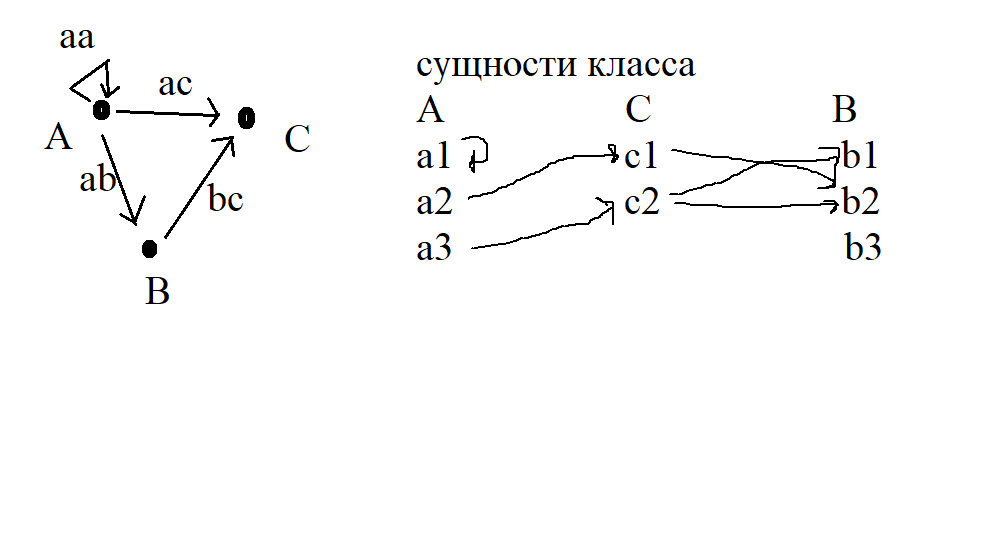
\includegraphics[scale=0.5]{example.png}
		\end{center}
	\end{figure}
	
	\normalsize
	\begin{verbatim}
	from ontology import *
	
	ont=Ontology()
	ont.addClass('A')
	ont.addClass('B')
	ont.addClass('CC')
	ont.addClass('D')
	ont.changeClass('CC','C')
	ont.deleteClass('D', True)
	print(ont.getAllClasses())# [A, B, C]
	
	ont.addRelationship('aa','A','A')
	ont.addRelationship('ab','A','B')
	ont.addRelationship('ac','A','C')
	ont.addRelationship('cb_','C','B')
	ont.addRelationship('bb','B','B')
	ont.changeRelationship('cb_','cb','C')
	ont.deleteRelationship('bb','B', False)
	
	ont.addEntity('a1','A')
	ont.addEntity('a2','A')
	ont.addEntity('b1','B')
	ont.addEntity('b2','B')
	ont.addEntity('b3','B')
	ont.addEntity('c1','C')
	ont.addEntity('c2_','C')
	ont.addEntity('c3','C')
	ont.changeEntity('c2_','c2','C')
	ont.deleteEntity('c3','C')
	
	ont.addEntityRelationship('aa','A','a1','a1')
	ont.addEntityRelationship('ac','A','a2','c1')
	ont.addEntityRelationship('ac','A','a2','c2')
	ont.addEntityRelationship('cb','C','c1','b2')
	ont.addEntityRelationship('cb','C','c2','b2')
	ont.addEntityRelationship('cb','C','c2','b1')
	ont.addEntityRelationship('cb','C','c2','b3')
	ont.deleteEntityRelationship('cb','C','c2','b3')
	
	print(ont.getAllClasses())# [A, B, C]
	print(ont.getAllRelationshipsForOutClass('A'))# [aa, ab, ac]
	print(ont.getAllRelationshipsForOutClass('B'))# []
	print(ont.getAllRelationshipsForOutClass('C'))# [cb]
	print(ont.getAllRelationshipsForOutClassToInClass('A','B'))# [ab]
	print(ont.getAllRelationshipsForOutClassToInClass('A','A'))# [aa]
	print(ont.getAllRelationshipsForOutClassToInClass('C','A'))# []
	print(ont.getAllEntitiesForClass('A'))# [a1, a2]
	print(ont.getAllEntitiesForClass('B'))# [b1, b2, b3]
	print(ont.getAllEntitiesForClass('C'))# [c1, c2]
	print(ont.getAllRelationshipedEntitiesForOutEntity('a1','A'))# [(A,a1)]
	print(ont.getAllRelationshipedEntitiesForOutEntity('a2','A'))# [(C,c1), (C,c2)]
	print(ont.getAllRelationshipedEntitiesForOutEntity('b1','B'))# []
	print(ont.getAllRelationshipedEntitiesForOutEntityForInClass('a2','A','C'))# [(C,c1), (C,c2)]
	print(ont.getAllRelationshipedEntitiesForOutEntityForInClass('a2','A','B'))# []
	print(ont.getAllRelationshipedEntitiesForOutEntityForRelationship('a2','A','ac'))# [(C,c1), (C,c2)]
	print(ont.getAllRelationshipedEntitiesForOutEntityForRelationship('a2','A','ab'))# []
	ont.saveToFile('ont1.txt')
	
	ont.loadFromFile('ont1.txt')
	#...
	ont.crear()
	ont=Ontology('ont1.txt')
	#...
	\end{verbatim}
	\large
\end{document}